% =====================================================================
%  Evolve — Evolvable Representations (research proposal)
%  Learning slow features that make fast evolutionary adaptation provably easy
%  Research proposal with first Stage-1 results. Author: Tom Offermann, ETH Zürich
% =====================================================================
\documentclass[11pt,a4paper]{article}

% ---------- layout & fonts ----------
\usepackage[a4paper,margin=2.4cm]{geometry}
\usepackage[T1]{fontenc}
\usepackage[utf8]{inputenc}
\IfFileExists{lmodern.sty}{\usepackage{lmodern}\usepackage{microtype}}{\usepackage[expansion=false]{microtype}}
\usepackage{parskip}
\usepackage{enumitem}
\setlist{itemsep=2pt,topsep=4pt}

% ---------- math ----------
\usepackage{amsmath,amssymb,amsthm,mathtools,bm}

% ---------- tables, figures, colors ----------
\usepackage{booktabs,tabularx,array,multirow}
\newcolumntype{L}[1]{>{\raggedright\arraybackslash}p{#1}}
\newcolumntype{Y}{>{\raggedright\arraybackslash}X}
\usepackage{xcolor}
\usepackage{graphicx}
\usepackage{caption}
\captionsetup{font=small,labelfont=bf}
\usepackage{tikz}
\usetikzlibrary{positioning,arrows.meta,shapes.geometric,shapes.misc,fit,backgrounds,calc,decorations.pathreplacing,shadows}
\usepackage{pgfplots}
\pgfplotsset{compat=1.18}
\usepgfplotslibrary{groupplots}
\usepackage[most]{tcolorbox}
\usepackage[ruled,vlined,linesnumbered]{algorithm2e}

% ---------- refs ----------
\usepackage[colorlinks=true,linkcolor=blue!50!black,citecolor=green!40!black,urlcolor=blue!60!black]{hyperref}
\usepackage[capitalise,noabbrev]{cleveref}

% ---------- palette ----------
\definecolor{slow}{HTML}{5B7FA6}     % frozen / gradient components
\definecolor{slowbg}{HTML}{E4ECF5}
\definecolor{fast}{HTML}{D9822B}     % evolutionary components
\definecolor{fastbg}{HTML}{FBEBDD}
\definecolor{mem}{HTML}{4E9A6B}      % memory / archive
\definecolor{membg}{HTML}{E2F1E7}
\definecolor{ink}{HTML}{333333}

% ---------- theorem environments ----------
\theoremstyle{definition}
\newtheorem{definition}{Definition}[section]
\newtheorem{example}[definition]{Example}
\theoremstyle{plain}
\newtheorem{proposition}[definition]{Proposition}
\newtheorem{lemma}[definition]{Lemma}
\newtheorem{conjecture}[definition]{Conjecture}
\theoremstyle{remark}
\newtheorem{remark}[definition]{Remark}

\newtcolorbox{keybox}[1][]{colback=fastbg,colframe=fast,boxrule=0.6pt,arc=2pt,left=6pt,right=6pt,top=4pt,bottom=4pt,fonttitle=\bfseries,#1}
\newtcolorbox{slowbox}[1][]{colback=slowbg,colframe=slow,boxrule=0.6pt,arc=2pt,left=6pt,right=6pt,top=4pt,bottom=4pt,fonttitle=\bfseries,#1}

% ---------- notation macros ----------
\newcommand{\R}{\mathbb{R}}
\newcommand{\N}{\mathbb{N}}
\newcommand{\E}{\mathbb{E}}
\IfFileExists{dsfont.sty}{\usepackage{dsfont}\newcommand{\one}{\mathds{1}}}{\newcommand{\one}{\mathbf{1}}}
\newcommand{\ind}[1]{\one\!\left[#1\right]}
\newcommand{\Dist}{\mathcal{D}}
\newcommand{\Ctx}{\mathcal{C}}
\newcommand{\Gen}{\mathcal{G}}          % genome space
\newcommand{\Lib}{\mathcal{E}}          % expert library
\newcommand{\Arch}{\mathcal{M}}         % archive
\newcommand{\RefSet}{\mathcal{R}}          % reference / few-shot set
\newcommand{\norm}[1]{\left\lVert #1 \right\rVert}
\newcommand{\ip}[2]{\left\langle #1, #2 \right\rangle}
\newcommand{\Ham}{\operatorname{Ham}}
\newcommand{\KL}{\operatorname{KL}}
\newcommand{\JS}{\operatorname{JS}}
\newcommand{\sg}{\operatorname{sg}}
\newcommand{\TopK}{\operatorname{TopK}}
\newcommand{\softmax}{\operatorname{softmax}}
\newcommand{\argmax}{\operatorname*{arg\,max}}
\newcommand{\argmin}{\operatorname*{arg\,min}}
\newcommand{\Var}{\operatorname{Var}}
\newcommand{\fast}[1]{\textcolor{fast}{#1}}
\newcommand{\slowc}[1]{\textcolor{slow}{#1}}
\newcommand{\memc}[1]{\textcolor{mem}{#1}}

% ---------- additional macros for this proposal ----------
\newcommand{\Task}{\mathcal{T}}
\newcommand{\Evo}{\operatorname{Evo}}
\newcommand{\Capa}{\operatorname{Cap}}
\newcommand{\sign}{\operatorname{sign}}

\title{\textbf{Evolvable Representations}\\[4pt]
\large Learning slow features that make fast, gradient-free evolutionary adaptation provably easy\\[2pt]
\normalsize\itshape Research proposal --- semester project / practical work, ETH Zürich}
\author{Tom Offermann\\ \small MSc Computer Science (Machine Intelligence, minor Theoretical Computer Science), ETH Zürich\\ \small\texttt{toffermann@ethz.ch}}
\date{Draft of \today}

\begin{document}
\maketitle

\begin{abstract}
\noindent
Deployed models should keep adapting, often from nothing more than a scalar reward. Evolutionary algorithms (EAs) are the natural tool for this regime: they need only fitness values, parallelise perfectly and handle discrete, non-differentiable decisions. They also come with runtime theory. For \emph{additive} fitness landscapes, a (1+1)~EA re-adapts after a change of $k$ positions in $O(n\log k)$ evaluations.
Whether a real adaptation problem is additive, however, is not a property of the task alone. It is a property of the \emph{representation} on which the evolved parameters act.
This proposal makes that representation the object of study. A slow, gradient-trained encoder feeds a tiny, discrete, evolved read-out (the \emph{genome}). We ask how the encoder must be shaped so that the fitness landscape seen by the EA is nearly additive, and related tasks have nearby optima.
We (i)~define the \emph{evolvability} of a representation as the expected number of reward evaluations an EA needs to move between related tasks; (ii)~prove that, for threshold read-outs over binary features, epistasis is bounded by feature co-activation near the decision threshold; (iii)~propose \emph{evolution-in-the-loop} meta-training, where an inner EA solves tasks and the encoder is updated by gradients at the genomes the EA found, regularised towards low epistasis; and (iv)~lay out a staged experimental plan from a synthetic task family with known ground truth to reward-only adaptation on real images, sized for CPU clusters and a single T4 GPU, with a direct scaling path to reward-only routing adaptation in mixture-of-experts language models. A first Stage-1 run confirms the premise: the discrete EA's speed depends strongly on the representation (by more than an order of magnitude), far more than CMA-ES does, and per-task epistasis predicts adaptation speed. It also shows that the current synthetic world is too easy to separate shaped from generic representations, which the experiments now running address.
\end{abstract}

\begin{keybox}[title={The question in one sentence}]
Meta-learning (MAML and friends) shapes representations so that \emph{gradient descent} adapts fast.
We ask the evolutionary counterpart: \textbf{what must a learned representation look like so that a simple EA, seeing only scalar rewards, adapts fast and provably so}, and can such a representation be \emph{trained}?
\end{keybox}

\tableofcontents
\newpage

% =====================================================================
\section{Motivation}
\label{sec:motivation}
% =====================================================================

\paragraph{Adaptation after deployment, from reward alone.}
A model that is deployed into a changing world rarely receives labelled gradients. It receives outcomes: a task succeeded or failed, a user accepted or rejected, a robot moved forward or fell over. In this \emph{reward-only} regime, gradient-based fine-tuning is either unavailable or requires high-variance estimators (policy gradients), and it moves all parameters at once, which causes forgetting.

\paragraph{Why evolutionary algorithms.}
EAs optimise any scalar objective, evaluate candidates in parallel, and handle discrete choices natively. Their weakness is dimension: in $n$ dimensions, a population of size $N$ yields a search direction whose signal fraction is only $N/(N+n+1)$. This is why they fail on $10^9$ parameters. The remedy, developed in our earlier working document, is a \emph{slow/fast split}. A large encoder is trained by gradients and then frozen; only a tiny genome of $n\approx 10^2$ discrete values, placed at the very end, is evolved. Placing it late also makes the population cheap: the encoder runs once per input and all $N$ genomes are evaluated on cached features.

\paragraph{The missing piece: the landscape is made by the representation.}
The runtime of an EA is governed by the \emph{structure} of its fitness landscape. On additive (OneMax-like) landscapes, a (1+1)~EA is fast and its behaviour is understood exactly. On rugged, epistatic landscapes (NK landscapes, needle-in-a-haystack), it can be exponentially slow.
In the slow/fast split, the landscape over the genome is $g \mapsto F_\tau(g;\phi)$. It depends on the task $\tau$ \emph{and on the encoder} $\phi$. The same task can be trivial for an EA on one representation and hopeless on another (\cref{fig:concept}).
Current practice picks $\phi$ for reasons unrelated to evolutionary adaptation (supervised pretraining, reconstruction, contrastive objectives), and then hopes.

\paragraph{This proposal.}
We make the representation's \emph{evolvability}, in the sense of evolutionary biology, the capacity to generate adaptive variation, an explicit, measurable and trainable quantity:
\begin{enumerate}[label=\textbf{C\arabic*}]
\item \textbf{Definition.} The evolvability of a representation is the expected number of reward evaluations an EA needs to adapt between related tasks (\cref{def:evo}). It decomposes into a \emph{ruggedness} term (epistasis) and a \emph{task-distance} term (how far apart the optima of related tasks lie).
\item \textbf{Theory.} For threshold read-outs over binary features, pairwise epistasis is bounded by the probability that both features are co-active \emph{and} the example lies near the decision threshold (\cref{lem:epistasis}). This turns a landscape property into a property of the features that can be regularised directly. Combined with classical runtime results, additive landscapes give $O(n\log k)$ re-adaptation (\cref{prop:reopt}).
\item \textbf{Method.} \emph{Evolution-in-the-loop} meta-training: an inner EA solves sampled tasks from rewards; the encoder is updated by gradients evaluated \emph{at the genomes the EA found}, plus an epistasis regulariser (\cref{sec:method}).
\item \textbf{Evaluation.} A staged plan, from a synthetic task family with known latent factors to reward-only adaptation on real images, with baselines that isolate each claim (\cref{sec:experiments}).
\end{enumerate}

\begin{figure}[t]
\centering
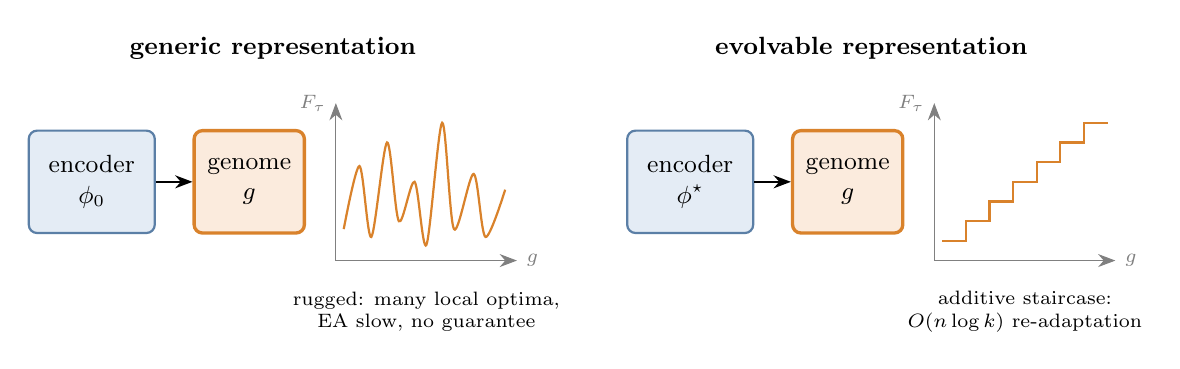
\begin{tikzpicture}[font=\small,>={Stealth[length=2.2mm]},
  slowblk/.style={draw=slow,fill=slowbg,rounded corners=3pt,thick,align=center,minimum height=1.3cm},
  fastblk/.style={draw=fast,fill=fastbg,rounded corners=3pt,very thick,align=center,minimum height=1.3cm}]
% ---------- left: unshaped ----------
\begin{scope}
\node[font=\small\bfseries] at (2.9,2.9) {generic representation};
\node[slowblk,minimum width=1.6cm] (e1) at (0.6,1.2) {encoder\\ $\phi_0$};
\node[fastblk,minimum width=1.4cm] (g1) at (2.6,1.2) {genome\\ $g$};
\draw[->,thick] (e1) -- (g1);
% rugged landscape
\draw[->,gray] (3.7,0.2) -- (6.0,0.2) node[right,font=\scriptsize,align=left]{$g$};
\draw[->,gray] (3.7,0.2) -- (3.7,2.2) node[left,font=\scriptsize]{$F_\tau$};
\draw[fast,thick,smooth] plot coordinates {(3.8,0.6) (4.0,1.4) (4.15,0.5) (4.35,1.7) (4.5,0.7) (4.7,1.2) (4.85,0.4) (5.05,1.95) (5.2,0.6) (5.45,1.3) (5.6,0.5) (5.85,1.1)};
\node[font=\scriptsize,align=center] at (4.85,-0.45) {rugged: many local optima,\\ EA slow, no guarantee};
\end{scope}
% ---------- right: shaped ----------
\begin{scope}[xshift=7.6cm]
\node[font=\small\bfseries] at (2.9,2.9) {evolvable representation};
\node[slowblk,minimum width=1.6cm] (e2) at (0.6,1.2) {encoder\\ $\phi^\star$};
\node[fastblk,minimum width=1.4cm] (g2) at (2.6,1.2) {genome\\ $g$};
\draw[->,thick] (e2) -- (g2);
\draw[->,gray] (3.7,0.2) -- (6.0,0.2) node[right,font=\scriptsize,align=left]{$g$};
\draw[->,gray] (3.7,0.2) -- (3.7,2.2) node[left,font=\scriptsize]{$F_\tau$};
\draw[fast,thick] (3.8,0.45) -- (4.1,0.45) -- (4.1,0.7) -- (4.4,0.7) -- (4.4,0.95) -- (4.7,0.95) -- (4.7,1.2) -- (5.0,1.2) -- (5.0,1.45) -- (5.3,1.45) -- (5.3,1.7) -- (5.6,1.7) -- (5.6,1.95) -- (5.9,1.95);
\node[font=\scriptsize,align=center] at (4.85,-0.45) {additive staircase:\\ $O(n\log k)$ re-adaptation};
\end{scope}
\end{tikzpicture}
\caption{\textbf{Same task, different landscape.} The fitness landscape an EA sees over the genome is determined jointly by the task and the frozen representation. This proposal trains the representation so that the landscape is close to additive, where EA runtime is fast and provable. (Schematic.)}
\label{fig:concept}
\end{figure}

% =====================================================================
\section{Setting and notation}
\label{sec:setting}
% =====================================================================

\subsection{Task family, encoder, genome}

\begin{center}
\small
\begin{tabularx}{\linewidth}{@{}lY@{}}
\toprule
\textbf{Symbol} & \textbf{Meaning} \\
\midrule
$\tau\sim P(\Task)$ & a task from a task family; $\Dist_\tau$ its distribution over $(x,y)$, $y\in\{-1,+1\}$ \\
$f_\phi:\mathcal{X}\to\{0,1\}^n$ & encoder with parameters $\phi$ producing $n$ binary features (the \slowc{slow} system) \\
$g\in\Gen=\{-1,0,1\}^n$ & ternary genome: each feature votes for, ignores, or votes against (the \fast{fast} system) \\
$m_g(x) = \ip{g}{f_\phi(x)} - \theta$ & read-out pre-activation with fixed threshold $\theta\notin\mathbb{Z}$ (no ties) \\
$\hat y_g(x) = \sign\, m_g(x)$ & prediction; $r_g(x,y) = \ind{y\, m_g(x) > 0}$ its correctness \\
$F_\tau(g;\phi) = \E_{\Dist_\tau}[r_g(x,y)]$ & fitness: expected reward (accuracy) of genome $g$ on task $\tau$ \\
$g^\star_\tau(\phi)$ & an optimal genome for $\tau$ under $\phi$ \\
$\mathcal{A}$ & an evolutionary algorithm that can only query (noisy estimates of) $F_\tau$ \\
$T_\mathcal{A}(g_0\to\tau;\phi)$ & number of fitness evaluations $\mathcal{A}$ needs, started at $g_0$, to reach $(1-\epsilon)\max_g F_\tau$ \\
$\Ham(g,g')$ & number of positions in which two genomes differ \\
\bottomrule
\end{tabularx}
\end{center}

The read-out is deliberately the simplest non-trivial one, a single ternary threshold unit (a perceptron with weights in $\{-1,0,1\}$), so that the landscape is a pseudo-Boolean-like function on a finite alphabet, the object that EA runtime theory studies. Multi-class and multi-output read-outs are obtained by stacking units with a fixed code (as in error-correcting output codes); every statement below then applies per unit.

\paragraph{Information available.}
\begin{itemize}
\item \textbf{Meta-training (offline, slow).} Labelled samples from a family of training tasks, as in standard meta-learning. The encoder may be trained with gradients.
\item \textbf{Deployment (online, fast).} For a new task, only the scalar batch reward $\hat F_\tau(g) = \frac1B\sum_{b} r_g(x_b,y_b)$ of each queried genome is observed. No labels, no gradients. This is the regime where an EA is the natural learner, rather than a worse replacement for gradient descent.
\end{itemize}

\begin{figure}[t]
\centering
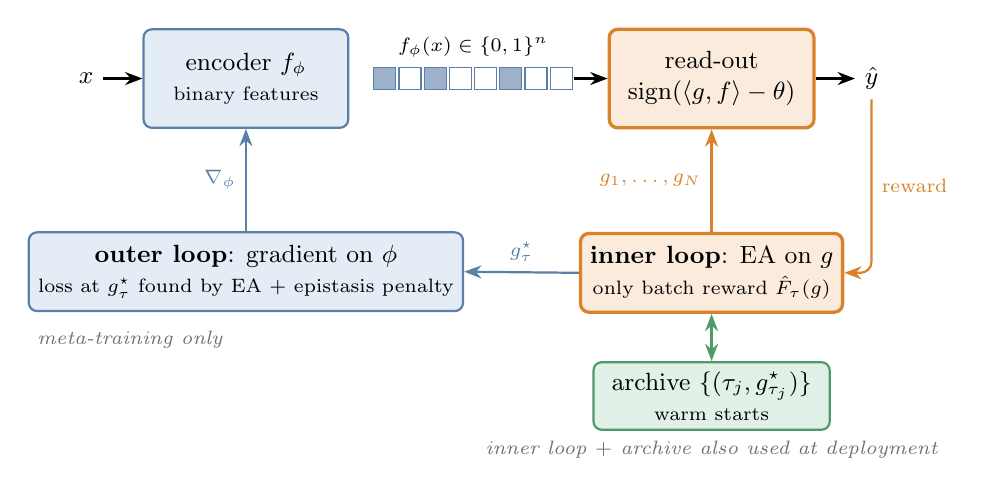
\begin{tikzpicture}[font=\small,>={Stealth[length=2.2mm]},
  slowblk/.style={draw=slow,fill=slowbg,rounded corners=3pt,thick,align=center,minimum height=1.25cm},
  fastblk/.style={draw=fast,fill=fastbg,rounded corners=3pt,very thick,align=center,minimum height=1.25cm},
  memblk/.style={draw=mem,fill=membg,rounded corners=3pt,thick,align=center}]
\node (x) at (0,0) {$x$};
\node[slowblk,minimum width=2.6cm,right=0.5cm of x] (enc) {encoder $f_\phi$\\ {\scriptsize binary features}};
% feature bits
\foreach \i/\c in {0/slow!60,1/white,2/slow!60,3/white,4/white,5/slow!60,6/white,7/white}{
  \node[draw=slow,fill=\c,minimum size=0.28cm,inner sep=0pt] at ($(enc.east)+(0.45+0.32*\i,0)$) {};
}
\node[font=\scriptsize] at ($(enc.east)+(1.57,0.4)$) {$f_\phi(x)\in\{0,1\}^n$};
\node[fastblk,minimum width=2.6cm] (ro) at ($(enc.east)+(4.6,0)$) {read-out\\ $\sign(\ip{g}{f}-\theta)$};
\draw[->,thick] (x) -- (enc);
\draw[->,thick] ($(enc.east)+(2.85,0)$) -- (ro);
\node[right=0.5cm of ro] (y) {$\hat y$};
\draw[->,thick] (ro) -- (y);
% inner loop
\node[fastblk,minimum width=3.3cm,minimum height=1.0cm,below=1.3cm of ro] (ea) {\textbf{inner loop}: EA on $g$\\ {\scriptsize only batch reward $\hat F_\tau(g)$}};
\draw[->,thick,fast] (ea.north) -- node[left,font=\scriptsize]{$g_1,\dots,g_N$} (ro.south);
\draw[->,thick,fast,rounded corners=4pt] (y.south) |- node[pos=0.25,right,font=\scriptsize]{reward} (ea.east);
% outer loop
\node[slowblk,minimum width=4.6cm,minimum height=1.0cm,below=1.3cm of enc] (outer) {\textbf{outer loop}: gradient on $\phi$\\ {\scriptsize loss at $g^\star_\tau$ found by EA $+$ epistasis penalty}};
\draw[->,thick,slow] (ea.west) -- node[above,font=\scriptsize]{$g^\star_\tau$} (outer.east);
\draw[->,thick,slow] (outer.north) -- node[left,font=\scriptsize]{$\nabla_\phi$} (enc.south);
% archive
\node[memblk,minimum width=3.0cm,minimum height=0.8cm,below=0.6cm of ea] (arch) {archive $\{(\tau_j,g^\star_{\tau_j})\}$\\ {\scriptsize warm starts}};
\draw[<->,thick,mem] (arch) -- (ea);
\node[font=\scriptsize\itshape,text=ink!70,anchor=west] at ($(outer.south west)+(0,-0.35)$) {meta-training only};
\node[font=\scriptsize\itshape,text=ink!70,anchor=north] at (arch.south) {inner loop $+$ archive also used at deployment};
\end{tikzpicture}
\caption{\textbf{Evolution in the loop.} A slow encoder produces binary features; a tiny ternary genome votes over them. During meta-training, an inner EA solves each sampled task from rewards only, and the encoder is updated by gradients evaluated at the genomes the EA found. At deployment, only the inner loop and the archive remain: adaptation is reward-only, parallel and leaves the encoder untouched.}
\label{fig:loop}
\end{figure}

\subsection{Evolvability of a representation}

Let $P(\tau,\tau')$ be a distribution over pairs of \emph{related} tasks (a task and its successor in a changing environment).

\begin{definition}[Capacity and evolvability]
\label{def:evo}
For an encoder $\phi$ and an EA $\mathcal{A}$,
\begin{align}
\Capa(\phi) &= \E_{\tau}\Big[\max_{g\in\Gen} F_\tau(g;\phi)\Big], \\
\Evo_\mathcal{A}(\phi) &= \E_{(\tau,\tau')\sim P}\Big[\,T_\mathcal{A}\big(g^\star_\tau(\phi)\to\tau';\ \phi\big)\Big].
\end{align}
$\Capa$ is what the representation \emph{can} express with a ternary vote; $\Evo$ is how many reward evaluations it costs to \emph{move} between related tasks. We seek representations with high capacity and low $\Evo$.
\end{definition}

The two quantities are in tension. The identity representation of raw pixels has low capacity for a single threshold unit. A representation with one feature per task ("grandmother cells") makes every task trivially solvable but relies on those tasks having been anticipated. The interesting regime lies in between: features that are \emph{reusable building blocks} of many tasks.

\subsection{Two knobs: ruggedness and task distance}

For single-position changes $\delta_i$ (setting $g_i$ to another value) define the first and second differences
\begin{equation}
\Delta_i F(g) = F(g\oplus\delta_i) - F(g),\qquad
\Delta^2_{ij} F(g) = F(g\oplus\delta_i\oplus\delta_j) - F(g\oplus\delta_i) - F(g\oplus\delta_j) + F(g).
\end{equation}
$F$ is \emph{additive} if all $\Delta^2_{ij}F\equiv 0$. We measure ruggedness by the \emph{relative epistasis}
\begin{equation}
\varepsilon_\tau(\phi) = \frac{\E_{g}\,\E_{i\neq j}\,\big|\Delta^2_{ij}F_\tau(g;\phi)\big|}{\E_g\,\E_i\,\big|\Delta_iF_\tau(g;\phi)\big|},
\end{equation}
with $g$ drawn along typical EA trajectories. The second knob is the \emph{task distance} $k_{\tau\tau'}(\phi) = \Ham\big(g^\star_\tau(\phi), g^\star_{\tau'}(\phi)\big)$: how many votes must change when the task changes.

\begin{proposition}[Re-adaptation on additive landscapes]
\label{prop:reopt}
Let $F$ be OneMax-like on $\{-1,0,1\}^n$, i.e.\ $F(g) = -\,|\{i: g_i\neq g^\star_i\}|$. The (1+1)~EA with per-position mutation probability $1/n$ (to a uniformly random other value), started at Hamming distance $k$ from $g^\star$, needs in expectation at most
\[
\E[T_k] \le 2\,e\,n\,H_k = O(n\log k)
\]
evaluations, where $H_k=\sum_{i=1}^k 1/i$.
\end{proposition}
\begin{proof}
At distance $i$, mutating exactly one of the $i$ wrong positions to its correct value, and nothing else, has probability at least $i\cdot\frac1n\cdot\frac12\cdot(1-\frac1n)^{n-1}\ge\frac{i}{2en}$. Elitism never increases the distance, so the expected waiting time at distance $i$ is at most $2en/i$; summing over $i=1,\dots,k$ gives the claim.
\end{proof}

\begin{remark}
Under exact additivity, $\Evo$ therefore scales like $n\,\E[\log k_{\tau\tau'}]$. A representation should thus make the landscape (nearly) additive, keep $n$ moderate, and make \emph{related tasks differ in few votes}. The last point echoes the biological finding that environments whose goals vary in a modular way produce modular, evolvable networks. For weighted additive functions over finite alphabets, $O(n\log n)$ bounds from arbitrary starting points are known; distance-$k$ bounds for weighted additive functions are an open question we intend to study (\cref{sec:rq}).
\end{remark}

% =====================================================================
\section{Where epistasis comes from: a feature-level bound}
\label{sec:theory}
% =====================================================================

The landscape of a threshold read-out is never exactly additive, because correctness is a step function of a sum. The following lemma says precisely \emph{where} the non-additivity comes from, and it only involves quantities that the encoder controls.

\begin{lemma}[Epistasis is co-activation near the threshold]
\label{lem:epistasis}
Let $f_\phi(x)\in\{0,1\}^n$, $g\in\{-1,0,1\}^n$, $m_g(x) = \ip{g}{f_\phi(x)}-\theta$ and $F(g) = \E[\ind{y\,m_g(x)>0}]$. Then for all $g$ and all single-position changes $\delta_i,\delta_j$ with $i\neq j$,
\begin{equation}
\big|\Delta^2_{ij}F(g)\big| \;\le\; 2\,\Pr_x\Big[f_i(x)=f_j(x)=1\ \text{ and }\ |m_g(x)| < 4\Big].
\end{equation}
\end{lemma}
\begin{proof}
Fix $(x,y)$ and write $a = (g_i'-g_i)f_i(x)$, $b = (g_j'-g_j)f_j(x)$ for the changes of the pre-activation caused by $\delta_i$ and $\delta_j$; note $|a|,|b|\le 2$. The per-example second difference is
$D = \rho(m+a+b)-\rho(m+a)-\rho(m+b)+\rho(m)$ with $\rho(t)=\ind{yt>0}$.
If $f_i(x)=0$ then $a=0$ and $D=\rho(m+b)-\rho(m)-\rho(m+b)+\rho(m)=0$; similarly if $f_j(x)=0$.
If $|m|> 4$, all four arguments $m, m+a, m+b, m+a+b$ lie on the same side of $0$ (since $|a+b|\le 4$, and $|m|=4$ is impossible because $\ip{g}{f}\in\mathbb{Z}$ and $\theta\notin\mathbb{Z}$), so $\rho$ is constant and $D=0$.
In all remaining cases $|D|\le 2$, since $D$ is a signed sum of four indicators with two positive and two negative signs. Taking expectations gives the bound.
\end{proof}

\begin{figure}[t]
\centering
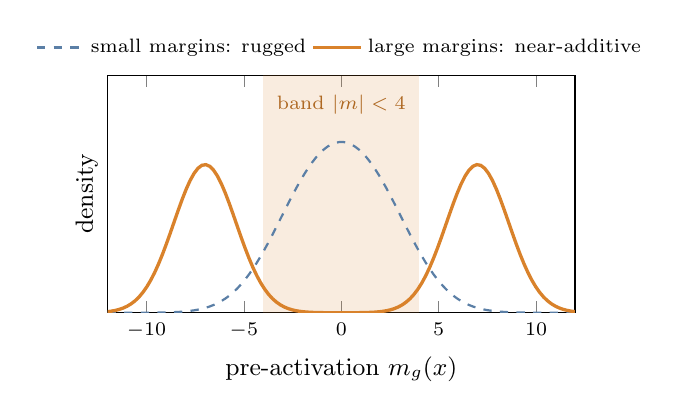
\begin{tikzpicture}
\begin{axis}[
  width=0.62\linewidth,height=4.6cm,
  xmin=-12,xmax=12,ymin=0,ymax=0.2,
  xlabel={pre-activation $m_g(x)$},ylabel={density},
  ytick=\empty,
  tick label style={font=\scriptsize},label style={font=\small},
  legend style={font=\scriptsize,draw=none,at={(0.5,1.03)},anchor=south,legend columns=2},
]
\fill[fast,opacity=0.15] (axis cs:-4,0) rectangle (axis cs:4,0.2);
\node[font=\scriptsize,text=fast!80!black] at (axis cs:0,0.175) {band $|m|<4$};
\addplot[slow,thick,dashed,domain=-12:12,samples=120] {0.5*exp(-(x-1.5)^2/(2*2.2^2))/(2.2*sqrt(2*pi)) + 0.5*exp(-(x+1.5)^2/(2*2.2^2))/(2.2*sqrt(2*pi))};
\addlegendentry{small margins: rugged}
\addplot[fast,very thick,domain=-12:12,samples=120] {0.5*exp(-(x-7)^2/(2*1.6^2))/(1.6*sqrt(2*pi)) + 0.5*exp(-(x+7)^2/(2*1.6^2))/(1.6*sqrt(2*pi))};
\addlegendentry{large margins: near-additive}
\end{axis}
\end{tikzpicture}
\hspace{0.6cm}
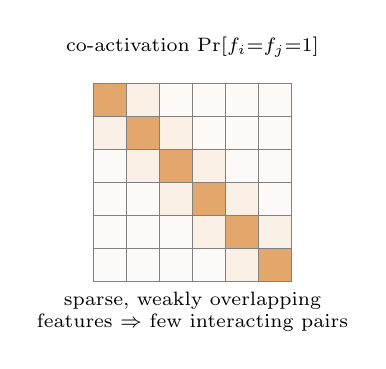
\begin{tikzpicture}[scale=0.42]
\node[font=\scriptsize,align=center] at (3,7.1) {co-activation $\Pr[f_i{=}f_j{=}1]$};
\foreach \i in {0,...,5}{\foreach \j in {0,...,5}{
  \pgfmathsetmacro{\v}{ifthenelse(\i==\j,70,ifthenelse(abs(\i-\j)==1,12,4))}
  \fill[fast!\v] (\j,5-\i) rectangle ++(1,1);
}}
\draw[gray] (0,0) grid (6,6);
\node[font=\scriptsize,align=center] at (3,-0.9) {sparse, weakly overlapping\\ features $\Rightarrow$ few interacting pairs};
\end{tikzpicture}
\caption{\textbf{The two feature-level sources of epistasis (\cref{lem:epistasis}), schematic.} Left: only examples whose pre-activation falls into the band $|m|<4$ can make two vote changes interact; large margins push mass out of the band. Right: only co-active feature pairs can interact; sparse, weakly overlapping features have few such pairs.}
\label{fig:lemma}
\end{figure}

\begin{remark}[Consequences]
\label{rem:consequences}
Summing over pairs, the total epistasis at $g$ satisfies
$\sum_{i\neq j}|\Delta^2_{ij}F(g)| \le 2\,\E\big[c(x)(c(x)-1)\,\ind{|m_g(x)|<4}\big]$, where $c(x)=\norm{f_\phi(x)}_1$ is the number of active features.
Two regimes make the landscape near-additive:
\begin{itemize}
\item \textbf{sparse regime}: few features active per input ($c(x)$ small), so few pairs can interact;
\item \textbf{margin regime}: most inputs far from the threshold, which requires \emph{many agreeing votes}, i.e.\ redundancy.
\end{itemize}
The two pull in opposite directions through $c(x)$. Which one a trained encoder chooses, and whether a mixture (sparse features with redundant copies) is optimal, is a concrete question the experiments can answer.
\end{remark}

\begin{remark}[Why a threshold read-out and not a linear one]
If per-example labels were available, a linear surrogate $\sum_b y_b\ip{g}{f(x_b)}$ would be maximised in closed form, and no EA would be needed. The EA earns its place exactly because deployment provides only scalar rewards, and the lemma shows that the non-linearity of the thresholded reward is \emph{local} (confined to the band and co-active pairs), so it can be controlled.
\end{remark}

% =====================================================================
\section{Method: evolution-in-the-loop meta-training}
\label{sec:method}
% =====================================================================

\subsection{Objective}

We train $\phi$ on a family of training tasks to maximise capacity while minimising the two drivers of $\Evo$:
\begin{equation}
\label{eq:objective}
\min_\phi\ \E_\tau\Big[\mathcal{L}_\tau\big(\phi;\,g^\star_\tau\big)\Big] \;+\; \lambda_{\text{co}}\,\mathcal{R}_{\text{co}}(\phi) \;+\; \lambda_{\text{band}}\,\E_\tau\,\mathcal{R}_{\text{band}}(\phi; g^\star_\tau),
\end{equation}
where $g^\star_\tau$ is the genome returned by the inner EA (treated as a constant), and
\begin{align}
\mathcal{L}_\tau(\phi;g) &= \E_{\Dist_\tau}\big[\max\big(0,\,\gamma - y\,\tilde m_g(x)\big)\big], & \tilde m_g(x) &= \ip{g}{\tilde f_\phi(x)}-\theta,\\
\mathcal{R}_{\text{co}}(\phi) &= \textstyle\sum_{i\neq j}\E_x\big[\tilde f_i(x)\tilde f_j(x)\big], &
\mathcal{R}_{\text{band}}(\phi;g) &= \E_{x}\big[\tilde c(x)^2\, \kappa\big(\tilde m_g(x)\big)\big].
\end{align}
Here $\tilde f_\phi = \sigma(h_\phi/T)$ are soft features (hard thresholding with a straight-through estimator at the end of training), $\tilde c = \norm{\tilde f}_1$, and $\kappa(t) = \sigma\big((4-|t|)/T\big)$ is a smooth indicator of the epistatic band. The hinge loss with margin $\gamma\ge4$ pushes examples out of the band on the task the genome solves; $\mathcal{R}_{\text{co}}$ targets the sparse regime, and $\mathcal{R}_{\text{band}}$ is the smooth version of the bound in \cref{rem:consequences}.

\subsection{Algorithm}

\begin{algorithm}[h]
\caption{Evolution-in-the-loop meta-training}
\label{alg:eil}
\KwIn{task family $P(\Task)$; encoder $f_\phi$; EA $\mathcal{A}$ with inner budget $T_{\text{in}}$; archive $\Arch=\emptyset$}
\For{outer step $s=1,2,\dots$}{
  sample tasks $\tau_1,\dots,\tau_M\sim P(\Task)$ (including successors $\tau'$ of earlier tasks)\;
  \For(\tcp*[f]{parallel over tasks}){$\tau\in\{\tau_1,\dots,\tau_M\}$}{
    $g_0\leftarrow$ best archived genome for a related task (or $0$)\;
    $g^\star_\tau\leftarrow\mathcal{A}(g_0;\ \hat F_\tau)$ with budget $T_{\text{in}}$, using only batch rewards on hard features\;
    record $T_\mathcal{A}$ and $\Ham(g_0,g^\star_\tau)$; store $(\tau,g^\star_\tau)$ in $\Arch$\;
  }
  $\phi\leftarrow\phi - \eta\,\nabla_\phi\Big[\frac1M\sum_\tau \mathcal{L}_\tau(\phi;g^\star_\tau) + \lambda_{\text{co}}\mathcal{R}_{\text{co}} + \lambda_{\text{band}}\frac1M\sum_\tau\mathcal{R}_{\text{band}}(\phi;g^\star_\tau)\Big]$\;
}
\end{algorithm}

The update is first-order: no gradient flows through the EA, exactly as in first-order MAML or Reptile. What makes it different from standard multi-task training is \emph{which} read-out the gradient is evaluated at: not a jointly trained linear head, but the discrete genome a black-box EA \emph{actually finds} within a small budget. The encoder is therefore pressured to make EA-reachable solutions good, which is a form of \emph{learning shaped by evolution}. It is the reverse direction of the Baldwin effect, where learning shapes evolution.

\subsection{Why this is cheap}
The inner loop acts on cached binary features: evaluating $N$ genomes on a batch of $B$ inputs is one $B\times n$ by $n\times N$ integer matrix product. With $n=64$, $B=512$ and $N=256$ this is $\approx 8\cdot10^6$ operations, i.e.\ microseconds to milliseconds on a CPU. The encoder is small in the synthetic stages and a fixed pretrained backbone plus a small trainable head in the real-image stage. The whole programme is sized for a CPU cluster (Euler) and a single T4 GPU.

% =====================================================================
\section{Research questions and hypotheses}
\label{sec:rq}
% =====================================================================

\begin{description}[leftmargin=1.2cm,style=nextline]
\item[RQ1] \textbf{Measurability.} Can $\varepsilon_\tau(\phi)$ and $k_{\tau\tau'}(\phi)$ be estimated reliably, and do they predict EA adaptation cost across representations?\\
\emph{H1: across encoders, $\log T_\mathcal{A}$ is well predicted by $\varepsilon$ and $\log k$.}
\item[RQ2] \textbf{Shapeability.} Does evolution-in-the-loop training reduce $\varepsilon$ and $k$ compared to generic representations of equal capacity?\\
\emph{H2: at matched $\Capa$, the shaped encoder has lower $\varepsilon$ and lower median $k$ than supervised multi-task, autoencoder and disentanglement-oriented encoders.}
\item[RQ3] \textbf{Payoff.} Does lower $\varepsilon$ translate into faster reward-only adaptation than strong gradient-free and policy-gradient baselines?\\
\emph{H3: evaluations to reach 95\% of the achievable reward drop by a large factor, and the drop grows with how related consecutive tasks are.}
\item[RQ4] \textbf{Theory.} How far do runtime guarantees extend beyond exact additivity?\\
\emph{Targets: distance-$k$ bounds for weighted additive functions on finite alphabets; bounds for the (1+1)~EA in terms of $\varepsilon$ or of the co-activation statistic of \cref{lem:epistasis}; which of the sparse and margin regimes is preferable.}
\end{description}

% =====================================================================
\section{Experimental plan}
\label{sec:experiments}
% =====================================================================

All stages share the protocol: meta-train on a family of tasks, then evaluate reward-only adaptation on \emph{held-out} tasks and task transitions. Every EA-based arm is run on every representation, so that the representation effect is isolated from the optimiser effect.

\subsection{Stage 1 --- synthetic task family with known ground truth (CPU)}

\begin{itemize}
\item \textbf{Generator.} Latent binary factors $s\in\{0,1\}^D$ ($D=16$), i.i.d.\ Bernoulli($\tfrac12$). Observations $x = M_2\tanh(M_1 s + \xi)\in\R^{64}$ with fixed random matrices $M_1,M_2$ and small noise $\xi$: an unknown non-linear entanglement of the factors.
\item \textbf{Tasks.} $y_\tau(s) = \sign\big(\sum_{j\in S_\tau} a_j(2s_j-1)\big)$ with $|S_\tau|=3$ and $a_j\in\{\pm1\}$. \emph{Related} successors change one element of $S_\tau$ or one sign, so the ground-truth change is small and known.
\item \textbf{Why it is useful.} The ideal representation is known (the factors themselves, possibly with redundant copies), so capacity, the achievable $k$, and the effect of shaping can be checked against ground truth.
\item \textbf{Encoder.} Two-layer MLP to $n\in\{32,64,128\}$ binary units.
\end{itemize}

\subsection{Stage 2 --- images with known factors (CPU / T4)}
dSprites or Shapes3D, whose generating factors (shape, scale, position, colour, \dots) are labelled. Tasks are sparse threshold rules over binarised factors, exactly as in Stage~1. Encoder: a small CNN. This stage tests whether shaping survives real perceptual input, and relates evolvability to disentanglement, which is measurable here.

\subsection{Stage 3 --- reward-only adaptation on natural images (T4)}
Frozen pretrained backbone (e.g.\ ResNet-18 or a small ViT) with cached features. The \emph{trainable} encoder is a small head mapping these features to $n$ binary units. Tasks are binary rules over CIFAR-100 classes, for example ``is it one of these three superclasses''. Successor tasks change one class group. Deployment sees only batch accuracy.

\subsection{Stage 4 --- scaling path (with large compute)}
\label{sec:scaling}
Stages 1--3 answer the scientific question on hardware available now (CPU cluster, one T4). With large compute, the same question transfers directly to language models, where reward-only adaptation is currently a central topic.
\begin{itemize}
\item \textbf{Slow system $=$ a mixture-of-experts LLM.} The ``features'' are the router inputs and the experts of the last $L'$ MoE layers (e.g.\ OLMoE, 64 experts per layer). The \textbf{genome} is a ternary or small-integer vector of per-expert routing biases $b_\ell\in\{-1,0,1\}^{K}$ (``force-exclude / neutral / prefer''), i.e.\ exactly the read-out of \cref{sec:setting}, one level up.
\item \textbf{Deployment:} reward-only domain adaptation, where the reward is the accuracy or verifier score on a batch of prompts from a new domain. The prompt prefix up to layer $L-L'$ is computed once and shared by the whole population, so evaluating $N$ genomes costs roughly one forward pass plus $N$ short suffixes.
\item \textbf{Shaping:} evolution-in-the-loop fine-tuning of the last-layer experts and routers. The inner EA finds routing genomes for training domains; the outer gradient updates experts and routers at those genomes, with the co-activation regulariser applied to expert co-selection (experts that are chosen together interact).
\item \textbf{Measurements} are unchanged: $\varepsilon$ and $k$ over routing genomes, evaluations to adapt, and comparisons with test-time routing methods (C3PO), policy-gradient fine-tuning (GRPO on LoRA) and ES fine-tuning of full weights (EGGROLL-style).
\item \textbf{Analogous instance:} a LoRA library in place of experts, with the genome as composition coefficients.
\end{itemize}
The small-scale stages are therefore not a toy detour. They build and validate the instruments ($\varepsilon$, $k$, evaluations-to-adapt, the lemma-derived regulariser) that the large-scale stage relies on.

\subsection{Arms}

\begin{center}
\small
\begin{tabularx}{\linewidth}{@{}lL{4.2cm}Y@{}}
\toprule
& arm & what it isolates \\
\midrule
\multicolumn{3}{@{}l}{\emph{Representations (each combined with the same EAs)}}\\
R0 & random binary projection & floor \\
R1 & supervised multi-task encoder (jointly trained linear heads, then binarised) & standard pretraining \\
R2 & autoencoder / $\beta$-VAE, binarised & reconstruction and disentanglement objectives \\
R3 & evolution-in-the-loop, $\lambda_{\text{co}}=\lambda_{\text{band}}=0$ & effect of training \emph{at EA-found genomes} alone \\
R4 & evolution-in-the-loop, full objective & \textbf{proposed} \\
R5 & R4 with randomised co-activation targets & control: regularisation vs.\ structure \\
\midrule
\multicolumn{3}{@{}l}{\emph{Adaptation algorithms at deployment (reward-only)}}\\
A1 & (1+1)~EA, ternary mutation & matches the theory \\
A2 & PBIL / cGA with population & parallel EA \\
A3 & CMA-ES on a continuous head over the same features & continuous gradient-free baseline \\
A4 & REINFORCE / ES on a continuous head & policy-gradient baseline \\
A5 & ES-MAML: meta-learned initialisation, ES adaptation & meta-learning for ES \\
A6 & ANIL-style head fine-tuning \emph{with labels} & reference upper bound, not reward-only \\
\bottomrule
\end{tabularx}
\end{center}

\subsection{Metrics}
\begin{itemize}
\item reward evaluations to reach $95\%$ of the task's achievable reward, for fresh tasks and for related successors;
\item $\varepsilon_\tau$, the distribution of $k_{\tau\tau'}$, and the co-activation and band statistics of \cref{lem:epistasis};
\item capacity $\Capa$ (achievable reward with a ternary vote) and final reward;
\item fit of adaptation time against $n\log k$ (slope and residuals) to test how far the additive theory carries;
\item stages~2--3: standard disentanglement scores, to relate evolvability to disentanglement.
\end{itemize}
Each configuration is run with at least 10 seeds. Controls get independent seeds, and every baseline's step size or learning rate is tuned. This follows lessons from earlier work in this project, where two conclusions were overturned by controls that could not vary.

\subsection{Compute and timeline}

\begin{center}
\small
\begin{tabularx}{\linewidth}{@{}lL{3.2cm}Y@{}}
\toprule
weeks & stage & deliverable \\
\midrule
1--2 & reading, generator, EA library & Stage-1 generator; (1+1)~EA/PBIL on cached binary features; $\varepsilon$ and $k$ estimators \\
3--5 & Stage 1 (Euler CPU) & RQ1 and RQ2 on ground truth; first go/no-go \\
6--8 & Stage 2 (CPU/T4) & shaping on dSprites/Shapes3D; link to disentanglement \\
9--11 & Stage 3 (T4) & reward-only adaptation vs.\ A3--A6 \\
12--14 & theory and write-up & RQ4 results; report \\
\midrule
later & Stage 4 (large compute) & MoE routing genomes and LoRA composition at LLM scale (\cref{sec:scaling}) \\
\bottomrule
\end{tabularx}
\end{center}

\paragraph{Go/no-go after Stage 1.} If, at matched capacity, R4 does not reduce $\varepsilon$ \emph{and} adaptation evaluations clearly below R1/R2, then shaping for evolvability does not work in the cleanest possible setting. The project then pivots to a measurement study (RQ1 and RQ4): which existing representations are evolvable, and why.

% =====================================================================
\section{Stage 1 in detail: protocol, first results, running experiments}
\label{sec:stage1}
% =====================================================================

This section specifies the Stage-1 experiment exactly as implemented (\path{research/evolvable/stage1/stage1_evolvable.py}, a single CPU-only file). It then reports a first two-seed run and states the experiments currently running, each with a decision rule fixed in advance.

\subsection{World and task family}
\begin{itemize}
\item \textbf{Latent factors} $s\in\{0,1\}^{D}$, $D=16$, i.i.d.\ Bernoulli$(\tfrac12)$.
\item \textbf{Observations} $x = M_2\tanh\big(M_1(2s-1)+b_1+\xi\big)\in\R^{64}$, where $M_1\in\R^{64\times16}$, $M_2\in\R^{64\times64}$ and $b_1$ are fixed Gaussian and $\xi\sim\mathcal{N}(0,0.05^2I)$. The factors are recoverable but non-linearly entangled.
\item \textbf{Tasks} $y_\tau(s)=\sign\big(\sum_{j\in S_\tau}a_j(2s_j-1)\big)$ with $|S_\tau|=3$ and $a\in\{\pm1\}^3$: $\binom{16}{3}\cdot 8 = 4480$ tasks. The sum is odd, so labels are never zero. A random 70\,\% of tasks is used for (meta-)training; the remaining 30\,\% are \emph{held out} and used only at evaluation.
\item \textbf{Related tasks} (successors) of $\tau$: flip one sign, or replace one factor of $S_\tau$ (with either sign). That gives 81 successors per task; for transitions we use successors that are themselves held out.
\end{itemize}

\subsection{Representations compared}
All learned encoders are the same MLP ($64\to128\to128\to n{=}64$, GELU) with binary outputs $f=\ind{h>0}$, trained with a straight-through estimator for 3000 steps (Adam).

\begin{center}
\small
\begin{tabularx}{\linewidth}{@{}lY@{}}
\toprule
name & training objective \\
\midrule
\texttt{ideal} & oracle: $f=[s,\,1-s,\,s,\,1-s]$ (true factors, both polarities, two copies) \\
\texttt{random} & untrained encoder (floor) \\
\texttt{autoencoder} & reconstruct $x$ from the binary code (MSE) \\
\texttt{multitask} & one linear head per training task (all 3136 heads every step, BCE); strong generic baseline \\
\texttt{multitask\_co} & \texttt{multitask} $+\;\lambda\,\mathcal{R}_{\text{co}}$ (plus a dead-unit guard) \\
\texttt{eil} & evolution in the loop (\cref{alg:eil}): 64 tasks per step, 30 inner (1+1)-EA iterations per task visit, persistent genome per task, hinge loss with $\gamma=1$ at the found genome \\
\texttt{eil\_full} & \texttt{eil} with margin $\gamma=4.5$ $+\;\lambda_{\text{co}}\mathcal{R}_{\text{co}}+\lambda_{\text{band}}\mathcal{R}_{\text{band}}$ \\
\texttt{eil\_margin}, \texttt{eil\_co} & ablations: only the margin, or only the co-activation penalty \\
\bottomrule
\end{tabularx}
\end{center}

\subsection{Adaptation protocol (reward only)}
For each seed and representation, $K=24$ held-out tasks are drawn. The draw is \emph{identical across representations}, so all comparisons are paired.
\begin{itemize}
\item \textbf{Reward:} accuracy on a fixed batch of 512 samples. All candidates of a run are evaluated on the same batch (common random numbers). Reported accuracy is on 4096 separate test samples.
\item \textbf{Fresh tasks:} search starts from the zero genome. \textbf{Transitions:} search for the successor $\tau'$ starts from the solution for $\tau$, after neutral drift has been pruned from it (below).
\item \textbf{Algorithms and budget:} 3000 reward evaluations per run.
  \begin{itemize}
  \item (1+1)~EA: mutation rate $1/n$ to a uniformly random other value; accepts ties; identical offspring are not evaluated.
  \item (1+16)~EA: forced mutation.
  \item CMA-ES on a continuous linear head (weights and bias) over the \emph{same} features, with restarts from the incumbent.
  \end{itemize}
\end{itemize}

\subsection{Metrics and statistics}
\begin{itemize}
\item \textbf{Speed:} reward evaluations until the best reward first reaches $0.90$ (censored at budget$+1$); evaluations to realise 95\,\% of the run's own improvement; the area under the best-so-far reward curve (AUC).
\item \textbf{Capacity:} held-out accuracy of the final genome, and of a logistic head trained \emph{with labels}. The latter is a reference only; it is not reward-only.
\item \textbf{Epistasis} $\varepsilon$: at four genomes along each (1+1) trajectory (after 64, 256 and 1024 evaluations, and the final one), 256 random pairs $(i,j)$ with random new values. $\varepsilon = \sum|\Delta^2_{ij}F| / \sum|\Delta_iF|$, computed on a separate 2048-sample batch (exact, no sampling noise).
\item \textbf{Lemma check:} for every such pair, $|\Delta^2_{ij}F|\le 2\Pr[f_i{=}f_j{=}1,\,|m|<4]$ is verified numerically.
\item \textbf{Task distance} $k$: positions of the final genome that differ from the start genome after \emph{pruning}. Pruning reverts every position whose reversion does not lower the reward (two sweeps), which removes neutral drift.
\item \textbf{Statistics:} paired Wilcoxon signed-rank tests over tasks $\times$ seeds (log evaluations, AUC); Spearman correlations for RQ1, pooled over non-oracle representations.
\end{itemize}

\paragraph{Correctness checks, run before every experiment.}
\begin{itemize}
\item Vectorised fitness equals a naive loop; labels are balanced.
\item The analytic ideal genome has accuracy $1$ on the oracle features.
\item The mutation operator moves a position to a uniformly random \emph{other} value.
\item The straight-through forward pass equals the hard bits.
\item \Cref{lem:epistasis} holds on random and oracle encoders.
\item The (1+1)~EA on OneMax-like ternary functions stays within the bound of \cref{prop:reopt}: the measured mean is 93--98\,\% of $2enH_k$ for $k\in\{1,4,16\}$, so the bound is nearly tight.
\end{itemize}

\subsection{First results (quick mode, 2 seeds, 48 paired tasks)}

\begin{table}[h]
\centering
\small
\begin{tabular}{@{}lccccccc@{}}
\toprule
& & \multicolumn{3}{c}{fresh held-out tasks} & \multicolumn{2}{c}{transitions} & \\
\cmidrule(lr){3-5}\cmidrule(lr){6-7}
representation & $\varepsilon$ & EA evals & CMA evals & EA test acc & EA evals & CMA evals & capacity (labels)\\
\midrule
\texttt{ideal} (oracle) & 0.58 & 144 & 158 & 1.000 & 84 & 132 & 1.000 \\
\texttt{random} & 0.72 & $>$3000 & $>$3000 & 0.707 & $>$3000 & $>$3000 & 0.755 \\
\texttt{autoencoder} & 0.67 & 2585 & 434 & 0.833 & $>$3000 & 453 & 0.975 \\
\texttt{multitask} & 0.63 & 176 & 159 & 0.986 & 111 & 161 & 1.000 \\
\texttt{multitask\_co} & \textbf{0.30} & 702 & 248 & 0.864 & 467 & 346 & 1.000 \\
\texttt{eil} & 0.65 & 690 & 352 & 0.883 & 594 & 461 & 0.948 \\
\texttt{eil\_full} & 0.63 & \textbf{170} & 172 & 0.985 & \textbf{96} & 192 & 1.000 \\
\bottomrule
\end{tabular}
\caption{\textbf{Stage 1, first run.} ``evals'' is the median number of reward evaluations to reach $0.90$; EA is the (1+1)~EA on the ternary genome, CMA is CMA-ES on a continuous head over the same features. All sanity checks passed; 0 lemma violations in all runs.}
\label{tab:stage1}
\end{table}

\begin{figure}[h]
\centering
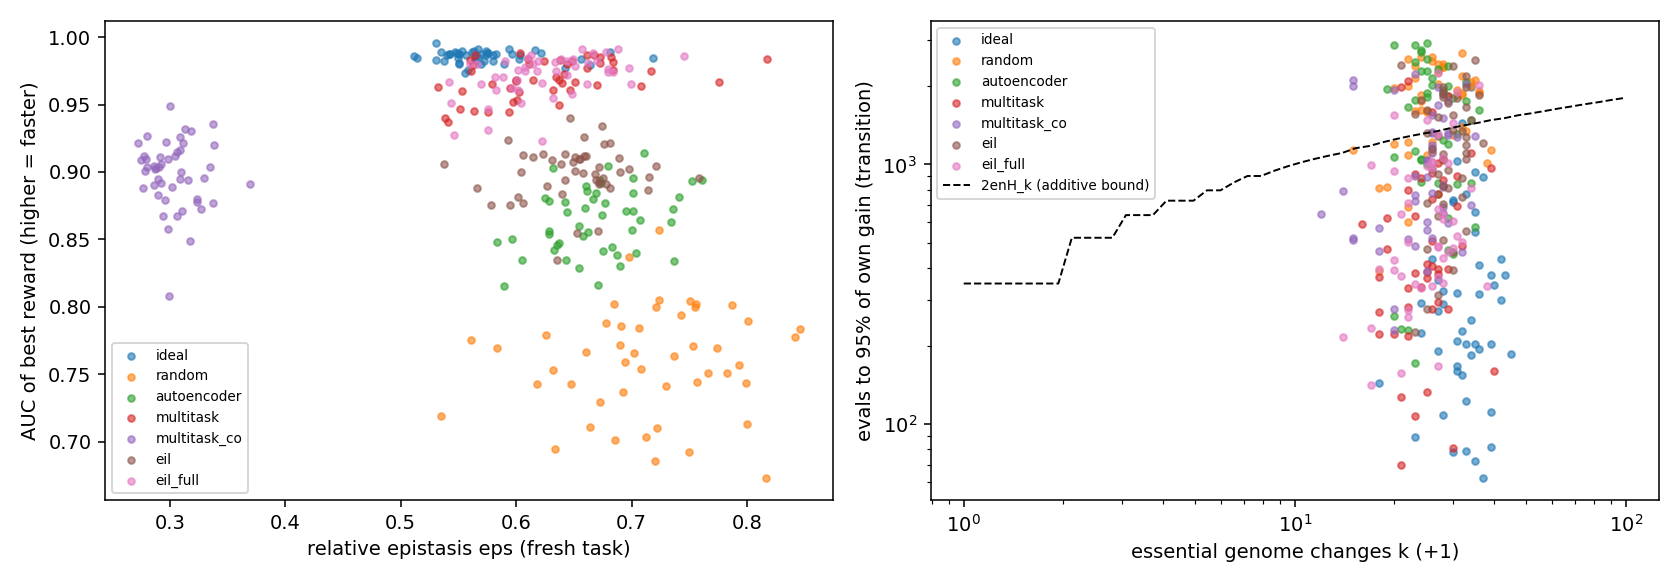
\includegraphics[width=\linewidth]{figures/stage1_rq1.png}
\caption{\textbf{RQ1, first run.} Left: relative epistasis vs.\ speed (AUC of best reward) per task. Right: essential genome changes $k$ vs.\ evaluations for transitions, with the additive bound $2enH_k$.}
\label{fig:stage1rq1}
\end{figure}

\paragraph{What the first run shows.}
\begin{enumerate}
\item \textbf{The benchmark cannot yet separate shaped from generic representations.}
\begin{itemize}
\item \texttt{eil\_full} vs.\ \texttt{multitask}: median ratio of evaluations $1.05$ ($p=0.91$) on fresh tasks and $0.97$ ($p=0.49$) on transitions.
\item Both are close to the oracle.
\item Supervised training on 3136 tasks already recovers the true factors, so this world cannot exhibit the failure that shaping targets. RQ2/RQ3 are therefore \emph{open}, not refuted.
\end{itemize}
\item \textbf{Evolution-in-the-loop details matter a lot.} \texttt{eil\_full} needs $4$--$7\times$ fewer evaluations than plain \texttt{eil} ($p<10^{-13}$, paired). The prime suspect is the margin term.
\item \textbf{Epistasis predicts speed, but it is not the whole story.}
\begin{itemize}
\item Per task, $\varepsilon$ correlates with speed: Spearman $\rho=-0.30$ (fresh) and $-0.41$ (transitions) against AUC, $p<10^{-6}$.
\item But \texttt{multitask\_co} halves $\varepsilon$ and still adapts $\approx4\times$ slower, because sparse features limit what a ternary vote can express.
\item The theory needs a second axis, \emph{read-out capacity}, next to epistasis.
\end{itemize}
\item \textbf{The discrete EA is far more sensitive to the representation than CMA-ES.}
\begin{itemize}
\item On good features, the ternary (1+1)~EA matches CMA-ES on fresh tasks and is about $2\times$ faster on transitions (\texttt{eil\_full}: 96 vs.\ 192 evaluations).
\item On autoencoder features it collapses (2585 vs.\ 434).
\item This directly supports the premise of the proposal: for evolutionary adaptation, the landscape is made by the representation.
\end{itemize}
\item \textbf{The small-$k$ regime is not reached.} Even on oracle features the EA finds dense genomes, and transitions change $\approx25$ positions where 2--4 would suffice. Sparse (parsimonious) search is needed to make the $O(n\log k)$ regime relevant.
\end{enumerate}

\subsection{Experiments currently running}
Each run tests one explanation for the first result. Its decision rule is fixed before seeing the outcome.

\begin{center}
\small
\begin{tabularx}{\linewidth}{@{}L{2.4cm}L{3.6cm}Y@{}}
\toprule
run & change & hypothesis and decision rule \\
\midrule
\textbf{Harder world} (\texttt{train\_frac}$=0.05$) & only $\approx224$ training tasks instead of 3136 & \emph{H:} with few tasks, multi-task training no longer recovers all factors, but evolution in the loop (which trains the features the EA can actually use) still does.
\emph{Supports RQ2/3} if \texttt{eil\_full} needs significantly fewer evaluations than \texttt{multitask} on held-out tasks (paired Wilcoxon $p<0.01$) at similar test accuracy. \emph{Against} if the two remain indistinguishable. \\
\textbf{Ablation} & \texttt{eil\_margin} (margin only) and \texttt{eil\_co} (co-activation only) & \emph{H:} the margin, i.e.\ the ``margin regime'' of \cref{rem:consequences}, explains the gain of \texttt{eil\_full} over \texttt{eil}.
\emph{Confirmed} if \texttt{eil\_margin} $\approx$ \texttt{eil\_full} and \texttt{eil\_co} $\approx$ \texttt{eil}. \\
\textbf{Stronger regularisers} ($\lambda_{\text{co}}=\lambda_{\text{band}}=1$) & $3\times$ larger penalties & \emph{H:} epistasis can be lowered substantially without losing capacity. It \emph{works} if $\varepsilon$ drops by $\ge30\,\%$ with test accuracy within $1$ point and no slow-down. It \emph{fails}, and confirms the capacity axis, if $\varepsilon$ drops and speed collapses as for \texttt{multitask\_co}. \\
\bottomrule
\end{tabularx}
\end{center}

\subsection{Round 1 outcomes}
Each run was judged by the decision rule stated above, before any interpretation. All tests are paired Wilcoxon over 48 tasks (2 seeds); ``evals'' is the median number of evaluations to reach $0.90$.

\begin{center}
\small
\begin{tabularx}{\linewidth}{@{}L{2.3cm}Y L{2.4cm}@{}}
\toprule
run & result & verdict \\
\midrule
Harder world & \textbf{Fresh tasks:} \texttt{eil\_full} 150 vs.\ \texttt{multitask} 202 evals ($0.74\times$, $p=0.0087$); AUC $p=5\cdot10^{-5}$; test accuracy 0.994 vs.\ 0.981. \textbf{Transitions:} 98 vs.\ 107 ($p=0.41$), AUC $p=2\cdot10^{-6}$. & supported on fresh tasks (weakly, 2 seeds) \\
Ablation & \texttt{eil\_margin} $\approx$ \texttt{eil\_full} ($p=0.32$); \texttt{eil\_co} $\approx$ \texttt{eil} ($p=0.09$); \texttt{eil\_margin} vs.\ \texttt{eil}: $0.30\times$ (fresh) and $0.17\times$ (transitions), $p<10^{-12}$ & confirmed: the margin does the work \\
Stronger regularisers & $\varepsilon$ only $-12\,\%$; $1.41\times$ slower ($p=7\cdot10^{-6}$); test accuracy $0.986\to0.943$ & fails as predicted; capacity axis confirmed \\
\bottomrule
\end{tabularx}
\end{center}

\paragraph{Interpretation.}
\begin{itemize}
\item \textbf{First separation.} In the harder world, the multi-task features remain \emph{equally informative}: the factors are perfectly decodable and a labelled logistic head is perfect. Yet the EA uses them less efficiently than features trained with evolution in the loop. This is the central claim in its cleanest form: good features for a gradient head are not the same as good features for an evolutionary head.
\item \textbf{The margin regime of \cref{lem:epistasis} is what matters, not the sparse regime.} Redundancy that pushes examples out of the band helps; lowering co-activation removes capacity.
\item \textbf{Relative epistasis $\varepsilon$ is not a valid predictor of adaptation cost.} Its correlation with speed changes sign across runs: $\rho=-0.30$, $+0.32$ and $+0.73$ against AUC. This is because regularisers lower $\varepsilon$ by sparsifying features, which also removes improving moves. RQ1 is therefore re-posed in terms of the first-order signal $\E|\Delta_iF|$ and the probability that a single mutation improves. Both are now measured.
\end{itemize}

\paragraph{Round 3 (running).}
\begin{itemize}
\item Five seeds of the harder world.
\item A tuned, compute-matched multi-task baseline: $4\times$ more steps, re-tuned head learning rate. This closes the two open caveats, rules 2 and 4 of our experimental practice.
\end{itemize}

\paragraph{Planned code extensions.} (i)~A \emph{parsimony tie-break}: among equal rewards, prefer fewer non-zero votes. This should give sparse genomes, small $k$, and the $O(n\log k)$ regime. (ii)~A held-out \emph{task-type} split: meta-train on 3-factor rules, evaluate on 5-factor rules and on unseen factor combinations. This makes generic training fail by construction, because the evaluation tasks are not in its training distribution.

% =====================================================================
\section{Related work}
\label{sec:related}
% =====================================================================

\paragraph{Evolvability.}
In evolutionary biology, evolvability is the capacity of a genotype--phenotype map to produce adaptive variation \cite{wagner1996complex}. Modularly varying goals make networks modular \cite{kashtan2005spontaneous}, and connection costs make them modular and more evolvable \cite{clune2013modularity}. In evolutionary computation, Evolvability ES directly optimises the behavioural diversity of a policy's offspring \cite{gajewski2019evolvability}. We transfer the concept to learned representations and make it quantitative through the landscape an EA sees over a late genome, with runtime-theoretic consequences.

\paragraph{Meta-learning.}
MAML learns an initialisation from which gradient steps adapt fast \cite{finn2017maml}. ANIL shows that most of MAML's benefit is feature reuse with a rapidly adapted head \cite{raghu2020anil}, the gradient counterpart of our slow encoder with a fast genome. ES-MAML replaces the inner gradient by ES \cite{song2020esmaml} and has been used for rapidly adaptable legged robots \cite{song2020rapidly}. Meta-learning through the Baldwin effect evolves initial parameters and hyperparameters for within-lifetime learning \cite{fernando2018baldwin}. All of these shape an \emph{initialisation} for a continuous inner learner; we shape the \emph{landscape} of a discrete, reward-only inner learner and target provable runtime.

\paragraph{Fitness landscapes and runtime theory.}
NK landscapes tune ruggedness through the degree of epistatic interaction \cite{kauffman1987walks}, and fitness--distance correlation predicts EA difficulty \cite{jones1995fdc}. The (1+1)~EA optimises linear pseudo-Boolean functions in $\Theta(n\log n)$ \cite{droste2002linear,witt2013tight}, also over finite alphabets \cite{doerr2012alphabet}; dynamic and re-optimisation settings have been studied for OneMax variants and linear functions \cite{kotzing2015dynamic,shi2019reopt}. We ask which learned representations make real adaptation problems fall into these tractable classes.

\paragraph{Representations and disentanglement.}
Disentangled representations aim to separate generative factors; their benefits and identifiability are debated \cite{locatello2019challenging}. Variance--covariance regularisation decorrelates features \cite{bardes2022vicreg}. Our co-activation regulariser is related, but it is \emph{derived} from an epistasis bound rather than posited, and it is evaluated by a downstream search cost.

\paragraph{Late evolved components and discrete masks.}
Evolving a small controller on top of learned models \cite{ha2018world}, gradient-free composition of adapters \cite{huang2024lorahub}, and selecting paths or binary masks over frozen networks for continual learning \cite{fernando2017pathnet,wortsman2020supsup} all place a small search problem on top of a fixed representation. None of them shape the representation for the search. Scaling ES to large models \cite{eggroll} is the complementary direction.

% =====================================================================
\section{Expected contributions and outlook}
% =====================================================================
\begin{enumerate}
\item A definition of evolvability for learned representations that is measurable and connects EA runtime theory to representation learning.
\item A feature-level epistasis bound for threshold read-outs, and theory on re-adaptation beyond exact additivity.
\item Evolution-in-the-loop meta-training, with evidence on whether it yields representations on which reward-only evolutionary adaptation is fast.
\item A benchmark suite of task families with known ground truth for studying evolutionary adaptation on learned features.
\end{enumerate}

\paragraph{Outlook.}
If representations can be made evolvable, the slow/fast split becomes a principled design for systems that keep adapting after deployment. The encoder is updated rarely and by gradients; the genomes adapt continuously from rewards, in parallel and without forgetting, stored in an archive that doubles as memory. The same question then applies to richer genomes: routing in mixtures of experts, or composition of adapter libraries.

% =====================================================================
\begin{thebibliography}{99}\small
\bibitem{bardes2022vicreg} A.~Bardes, J.~Ponce, Y.~LeCun. VICReg: variance-invariance-covariance regularization for self-supervised learning. ICLR 2022. arXiv:2105.04906.
\bibitem{clune2013modularity} J.~Clune, J.-B.~Mouret, H.~Lipson. The evolutionary origins of modularity. Proc.\ R.\ Soc.\ B 280, 2013. arXiv:1207.2743.
\bibitem{doerr2012alphabet} B.~Doerr, S.~Pohl. Run-time analysis of the (1+1) evolutionary algorithm optimizing linear functions over a finite alphabet. GECCO 2012.
\bibitem{droste2002linear} S.~Droste, T.~Jansen, I.~Wegener. On the analysis of the (1+1) evolutionary algorithm. Theoretical Computer Science 276, 2002.
\bibitem{eggroll} Evolution strategies at the hyperscale (EGGROLL). arXiv:2511.16652, 2025.
\bibitem{fernando2017pathnet} C.~Fernando et al. PathNet: evolution channels gradient descent in super neural networks. arXiv:1701.08734, 2017.
\bibitem{fernando2018baldwin} C.~Fernando et al. Meta-learning by the Baldwin effect. GECCO 2018 companion. arXiv:1806.07917.
\bibitem{finn2017maml} C.~Finn, P.~Abbeel, S.~Levine. Model-agnostic meta-learning for fast adaptation of deep networks. ICML 2017. arXiv:1703.03400.
\bibitem{gajewski2019evolvability} A.~Gajewski, J.~Clune, K.~O.~Stanley, J.~Lehman. Evolvability ES: scalable and direct optimization of evolvability. GECCO 2019. arXiv:1907.06077.
\bibitem{ha2018world} D.~Ha, J.~Schmidhuber. Recurrent world models facilitate policy evolution. NeurIPS 2018. arXiv:1803.10122.
\bibitem{huang2024lorahub} C.~Huang et al. LoraHub: efficient cross-task generalization via dynamic LoRA composition. COLM 2024. arXiv:2307.13269.
\bibitem{jones1995fdc} T.~Jones, S.~Forrest. Fitness distance correlation as a measure of problem difficulty for genetic algorithms. ICGA 1995.
\bibitem{kashtan2005spontaneous} N.~Kashtan, U.~Alon. Spontaneous evolution of modularity and network motifs. PNAS 102(39), 2005.
\bibitem{kauffman1987walks} S.~Kauffman, S.~Levin. Towards a general theory of adaptive walks on rugged landscapes. Journal of Theoretical Biology 128, 1987.
\bibitem{kotzing2015dynamic} T.~Kötzing, A.~Lissovoi, C.~Witt. (1+1) EA on generalized dynamic OneMax. FOGA 2015.
\bibitem{locatello2019challenging} F.~Locatello et al. Challenging common assumptions in the unsupervised learning of disentangled representations. ICML 2019. arXiv:1811.12359.
\bibitem{raghu2020anil} A.~Raghu, M.~Raghu, S.~Bengio, O.~Vinyals. Rapid learning or feature reuse? Towards understanding the effectiveness of MAML. ICLR 2020. arXiv:1909.09157.
\bibitem{shi2019reopt} F.~Shi, M.~Schirneck, T.~Friedrich, T.~Kötzing, F.~Neumann. Reoptimization time analysis of evolutionary algorithms on linear functions under dynamic uniform constraints. Algorithmica 81, 2019.
\bibitem{song2020esmaml} X.~Song et al. ES-MAML: simple Hessian-free meta learning. ICLR 2020. arXiv:1910.01215.
\bibitem{song2020rapidly} X.~Song et al. Rapidly adaptable legged robots via evolutionary meta-learning. IROS 2020. arXiv:2003.01239.
\bibitem{wagner1996complex} G.~P.~Wagner, L.~Altenberg. Complex adaptations and the evolution of evolvability. Evolution 50(3), 1996.
\bibitem{witt2013tight} C.~Witt. Tight bounds on the optimization time of a randomized search heuristic on linear functions. Combinatorics, Probability and Computing 22, 2013.
\bibitem{wortsman2020supsup} M.~Wortsman et al. Supermasks in superposition. NeurIPS 2020. arXiv:2006.14769.
\end{thebibliography}

\end{document}
